\chapter{Plataforma de desarrollo}
\label{cap:capitulo4}

\begin{flushright}
\begin{minipage}[]{10cm}
\emph{Las herramientas adecuadas en las manos adecuadas pueden cambiar el mundo}\\
\end{minipage}\\
Steve Jobs\\
\end{flushright}

\vspace{1cm}
Tras haber establecido los objetivos que se pretenden alcanzar en este trabajo de fin de grado, se procede a describir
las herramientas \textit{software} y \textit{hardware} utilizadas para lograrlos. 

\section{Software}
\label{sec:software}
Llamamos \textit{software} al conjunto de programas, instrucciones y datos que dotan de lógica a un sistema.
\subsection{Python}
\label{subsec:pyhton}
\noindent Python es un lenguaje de programación interpretado de alto nivel. Cuando se dice que un lenguaje es de alto nivel, se hace referencia a su nivel de 
abstracción y facilidad de uso en comparación con los lenguajes de bajo nivel, es decir, aquellos que te permiten mayor control sobre los 
componentes físicos del sistema. Decimos que es un lenguaje interpretado debido a que no es necesario convertir el texto escrito por el humano en 
instrucciones entendibles por un procesador previamente a su ejecución.  

Una de las características más destacadas de Python es su amplia librería\footnote{conjunto de código destinado a un objetivo concreto} estándar, que proporciona 
una gran variedad de módulos y funciones para realizar multitud de tareas. Además, como cualquier otro lenguaje de programación, cuenta con una gran cantidad de librerías de terceros que 
amplían sus capacidades, como SciPy en la ciencia de datos, Django en el desarrollo web, Numpy para operar con matrices, TensorFlow el aprendizaje automático, entre otros.

\subsection{Grbl}
\label{subsec:grbl}
\noindent Grbl\footnote{\url{https://github.com/gnea/grbl}} es un \textit{firmware}\footnote{software específico para el harware elegido} de código abierto utilizado para controlar máquinas \acs{CNC}. 
Está pensado para poderse ejecutar en microcontroladores de bajos recursos, como pueden ser los Arduinos y los ESP32.

Básicamente, convierte una serie de instrucciones de código G (posteriormente se hablará de él) en señales eléctricas que se envían a 
los motores de la máquina. Además de eso, comprueba los sensores de la máquina, para poder conocer y establecer los límites físicos de cada movimiento. 

Grbl es flexible por lo que podemos cambiar la configuración para adaptarla a un caso de uso concreto. De hecho, aunque principalmente está pensado para realizar 
movimientos lineales, en este trabajo se abordará la configuración necesaria para poder usarse en articulaciones rotativas.
\begin{figure} [h!]
  \begin{center}
    
\includegraphics[width=4cm]{figs/grbl.png}
  \end{center}
  \caption{Logo de Grbl}
  \label{fig:grbllogo}
\end{figure}\ 
\subsection{Código G}
\label{sec:gcode}
\noindent \textit{G-code}, también conocido como RS-274, es el nombre del lenguaje de programación más usado en máquinas de \ac{CNC}. 

Su programación, precisa de una sintaxis específica en la que se emplean letras y números para representar 
diferentes comandos y parámetros. Por ejemplo, la letra G seguida de un número indica un comando de movimiento, mientras 
que la letra M seguida de un número se utiliza para comandos misceláneos, como el encendido o apagado del láser.
En el Código \ref{cod:ejemplo_gcode} se muestra un ejemplo muy sencillo, para trazar un cuadrado de 20mm de lado.

\begin{code}[h]
\begin{verbatim}
  G90       ; Establecer modo de posicionamiento absoluto
  G21       ; Establecer unidad de medida en milímetros
  F200      ; Establecer velocidad de avance a 200 unidades por minuto 
  
  G0 X0 Y0  ; Mover a la posición inicial (esquina inferior izquierda) 
  G1 X20    ; Mover horizontalmente hacia la derecha 20 mm
  G1 Y20    ; Mover verticalmente hacia arriba 20 mm
  G1 X0     ; Mover horizontalmente hacia la izquierda 20 mm
  G1 Y0     ; Mover verticalmente hacia abajo 20 mm
  G0 X0 Y0  ; Volver a la posición inicial (esquina inferior izquierda)
  
  M2        ; Fin del programa
\end{verbatim}
\caption{Programa para realizar una trayectoria cuadrada}
\label{cod:ejemplo_gcode}
\end{code}
\newpage
\subsection{FreeCAD}
\label{subsec:freecad}
\noindent FreeCAD\footnote{\url{https://www.freecad.org/index.php?lang=es_ES}} es un programa de diseño asistido por ordenador de código abierto y gratuito, 
utilizado para modelar piezas industriales.
Está dirigido al mundo de la ingeniería mecánica y el diseño de productos.

Utiliza el enfoque del modelado paramétrico, que se basa 
en el uso de parámetros y relaciones entre ellos para construir modelos 3D que pueden ser 
modificados fácilmente. 

Una de las ventajas de FreeCAD es la disponibilidad de diversos bancos de trabajo especializados, 
conocidos como \textit{workbenches}. Cada uno de ellos, proporciona herramientas y funciones 
específicas para tareas de diseño particulares.

Además, es altamente personalizable, ya que incorpora un administrador de complementos que permite a la comunidad 
agregar nuevas herramientas y funcionalidades al software. Gracias a ella, el software mejora continuamente y 
resulta sencillo de aprender debido a la cantidad de documentación y tutoriales que existen.

\begin{figure} [h!]
  \begin{center}
    
\includegraphics[width=4cm]{figs/freecad.png}
  \end{center}
  \caption{Logo de FreeCAD}
  \label{fig:freecadlogo}
\end{figure}\ 
\newpage
\subsection{ROS 2}
\label{subsec:ros2}
\noindent ROS, por sus siglas en inglés, significa \textit{Robot Operating System}. Se trata de una plataforma de código abierto utilizada 
para desarrollar y controlar sistemas robóticos.

Su objetivo principal es facilitar el desarrollo de sistemas robóticos al proporcionar una infraestructura que permite a
los desarrolladores centrarse en la lógica y el comportamiento específico de los robots, sin tener que preocuparse por la 
infraestructura de comunicación y control. 

Sumado a ello, proporciona una colección de bibliotecas, herramientas y convenios que permiten a los desarrolladores 
reutilizar y modularizar el software para robots. Además, incorpora programas para la visualización de datos, depuración y 
simulación de robots creados por una comunidad activa de usuarios y desarrolladores.

Una de las características distintivas de ROS es su arquitectura basada en nodos. Los nodos son procesos independientes 
que se comunican entre sí mediante mensajes. Cada nodo puede realizar tareas específicas, en función de la lógica atribuida por el programador.

Concretamente, en este trabajo se utiliza ROS 2, la versión sucesora de ROS. Esta versión incorpora una gran variedad de mejoras respecto 
a su predecesor. Por ejemplo, los nodos no dependen de un componente \textit{Master} para comunicarse ya que las comunicaciones 
están distribuidas mediante el uso de \ac{DDS}. Esto incrementa la robustez del sistema y reduce significativamente los tiempos de latencia. 

La distribución de ROS utilizada en este trabajo es \textit{ROS 2 Humble}. Se trata de la última versión de ROS estable disponible para 
el sistema operativo Ubuntu 22.04 LTS.
\begin{figure} [h!]
  \begin{center}
    
\includegraphics[width=4cm]{figs/ros2logo.jpeg}
  \end{center}
  \caption{Logotipo de ROS 2 Humble}
  \label{fig:ros2logo}
\end{figure}\ 

\subsection{MoveIt!}
\label{subsec:moveit}
MoveIt es una plataforma de desarrollo (\textit{framework}) de código abierto que permite implementar 
aplicaciones de manipulación complejas utilizando ROS. 

Además, proporciona una amplia gama de herramientas y bibliotecas que 
facilitan el control y la planificación de movimientos. Con este software, se puede desarrollar fácilmente aplicaciones que permitan
a los robots realizar tareas de manipulación avanzadas, como agarrar objetos, ensamblar piezas y maniobrar el brazo en entornos complejos. 

Es altamente flexible gracias a su diseño modular y se puede utilizar con una gran variedad de robots. De hecho, incorpora la herramienta 
\textit{MoveIt Setup Assistant}, que se trata de un asistente de configuración con interfaz gráfica, que te permite generar los ficheros 
necesarios para poder incorporar tu propio robot en este ecosistema. 
\begin{figure} [h!]
  \begin{center}
    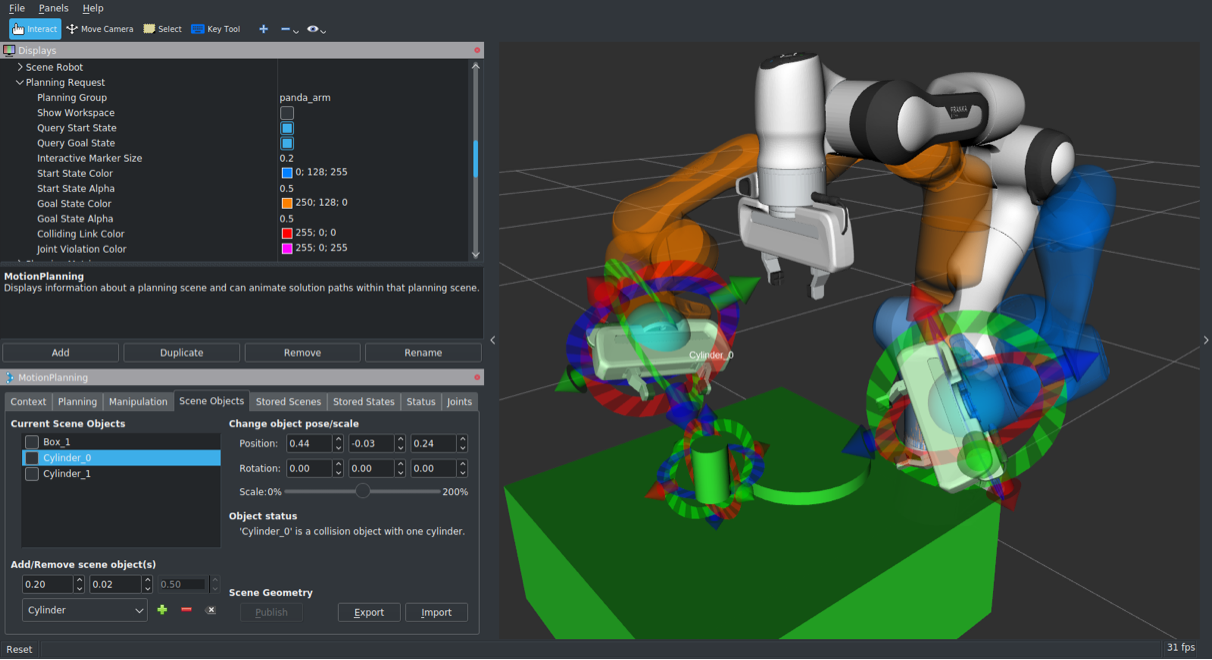
\includegraphics[width=14cm]{figs/moveit_intro.png}
  \end{center}
  \caption{Plugin de MoveIt para el visualizador de ROS, Rviz2 (Franka Emika Robot)}
  \label{fig:ros2logo}
\end{figure}\ 

\newpage
\section{Hardware}
\label{sec:hardware}
Cuando hablamos de \textit{hardware}, nos referimos a todos los componentes físicos de utilizados en el dispositivo electrónico, en este caso, el robot. Estos 
componentes son tangibles, es decir, se pueden tocar y ver.

\subsection{MKS DLC32}
\label{subsec:mksdlc32}
\noindent Se trata de una placa base\footnote{componente esencial que proporciona conexiones y circuitos para que los demás componentes se comuniquen entre sí} destinada al mundo de las máquinas de grabado láser. 

Ha sido creada por \textit{MakerBase} y es \textit{open hardware}, por lo que toda la información de la placa 
puede encontrarse en su repositorio de Github\footnote{\url{https://github.com/makerbase-mks/MKS-DLC32}}. Aun así, es fácil de comprar 
en páginas web como \textit{Aliexpress} por un precio que ronda los 16\euro. 

Está basada en el 
microcontrolador ESP32. Éste, es un dispositivo muy asentado en la comunidad \textit{maker} debido a su bajo coste e integración en el 
ecosistema Arduino que, sumado a su a su conectividad wifi, es una opción cada vez más popular entre los fabricantes de este tipo de placas.

Como cabe esperar, es compatible con \nameref{subsec:grbl} e incorpora una serie de características que la hacen ideal para este proyecto. Es capaz de 
controlar hasta 3 motores junto con una señal de \acs{PWM} para añadirle un servomotor, electroimán o láser.
\begin{figure} [h!]
    \begin{center}
      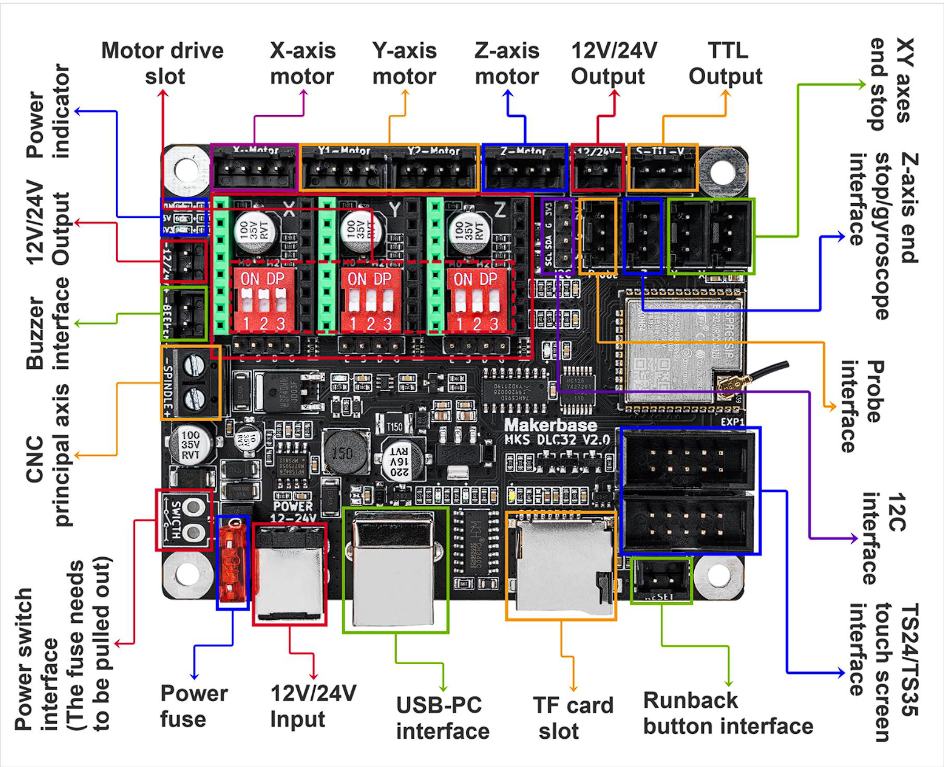
\includegraphics[width=9cm]{figs/MKS.png}
    \end{center}
    \caption{Placa base MakerBase DLC32}
    \label{fig:robSoldering}
  \end{figure}\ 

\subsection{Motores Nema 17}
\label{subsec:motores}
\noindent Un motor paso a paso es un tipo de motor que se mueve en pequeños incrementos discretos en lugar de girar continuamente. Esta  
posibilidad de tener un control sobre la rotación del motor hace que sea la opción idónea para mover las articulaciones del robot.

Concretamente, se han usado 3 motores Nema 17 de 60 milímetros de largo como los mostrados en la Figura \ref{fig:nema17_60}. Se tratan de
motores bipolares de 2.1 amperios y una resistencia de 1,6 ohmios con un torque máximo de 0.65 newton-metro. Estos, han sido comprados 
en \textit{Amazon} por un precio de 55\euro. 

En la Tabla \ref{cuadro:nema17_60} 
se muestran las especificaciones técnicas de los motores elegidos
\begin{figure} [h!]
    \begin{center}
      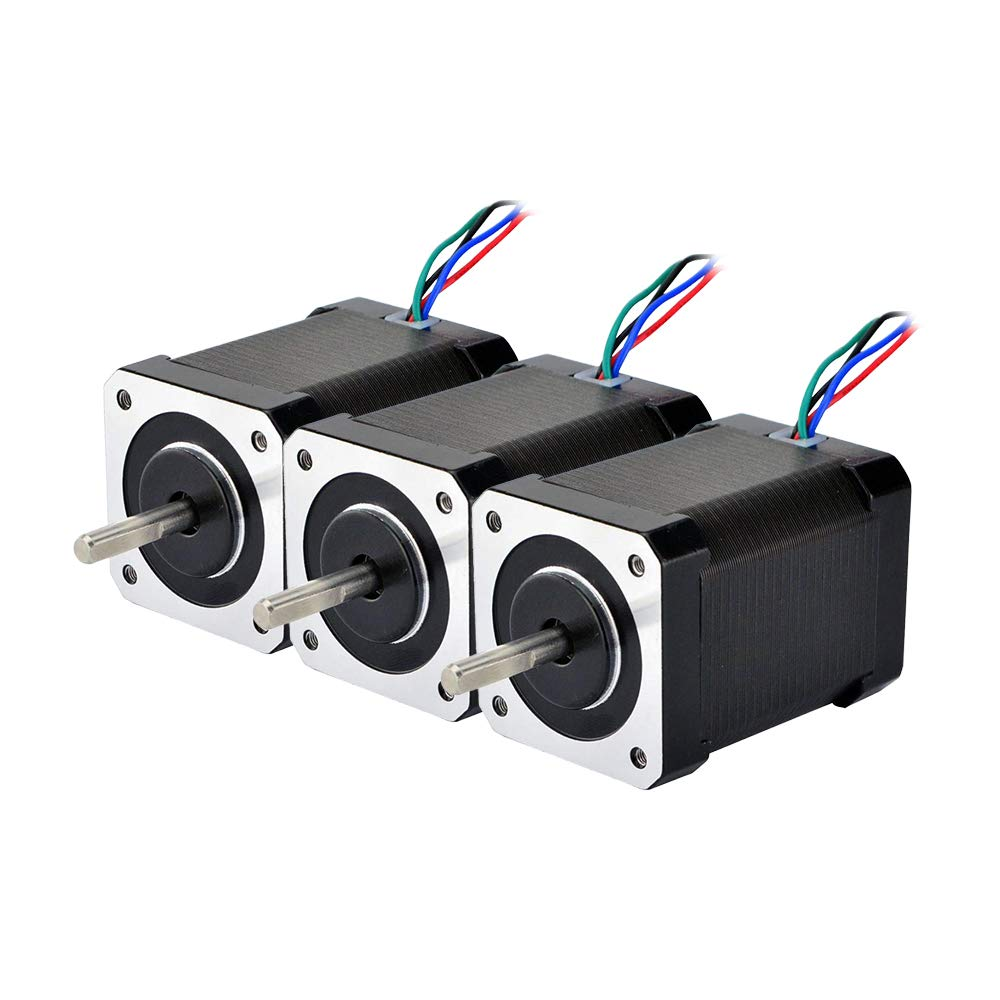
\includegraphics[width=9cm]{figs/nema17.jpg}
    \end{center}
    \caption{Motores Nema 17 de 2.1A}
    \label{fig:nema17_60}
  \end{figure}\ 

\begin{table}[H]
\begin{center}
\begin{tabular}{|c|c|}
\hline
\textbf{Parámetros} & \textbf{Valores} \\
\hline
Nombre del motor & 17HS24-2104S \\
Tipo de motor & Bipolar \\
Ángulo de paso & 1.8º \\
Resistencia de fase & 1.6$\Omega$ \\
Corriente máx. de fase & 2.1A \\
Torque de sujeción & 0.65Nm. \\
Dimensiones & 42x42x60mm \\
Peso & 500g \\
Diámetro del eje & 5mm \\
Longitud del eje & 24mm \\
\hline
\end{tabular}
\caption{Especificaciones técnicas de los motores utilizados}
\label{cuadro:nema17_60}
\end{center}
\end{table}

\newpage
\subsection{Controlador TMC2209}
\label{subsec:controladorPAP}
\noindent Un controlador paso a paso es el módulo hardware capaz de trasformar las señales lógicas que le envía el procesador, en una serie de pulsos de
potencia que excitarán ambas bobinas del motor en un cierto orden para hacerlo girar. 
En concreto, se han utilizado 3 controladores TMC2209, compatibles con la placa mencionada anteriormente. Este modelo específico, es capaz 
de entregar mayor corriente que su competencia e incluye una serie de tecnologías que reducen el ruido en los motores y las vibraciones. Además, 
cuenta con una serie de protecciones para evitar dañarse en caso de un mal uso. Aún con todo esto, su precio por unidad es de apenas 3\euro.
\begin{figure} [h!]
    \begin{center}
      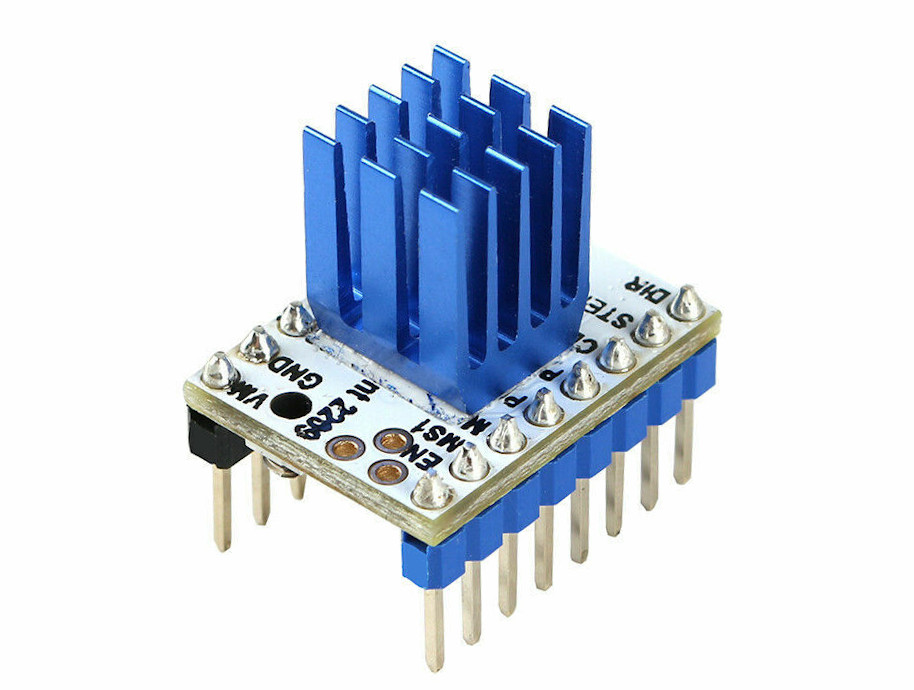
\includegraphics[width=8cm]{figs/TMC2209.jpg}
    \end{center}
    \caption{Controlador TMC2209}
    \label{fig:robSoldering}
\end{figure}\ 

\begin{table}[H]
\begin{center}
\begin{tabular}{|c|c|}
\hline
\textbf{Parámetros} & \textbf{Valores} \\
\hline
Nombre del controlador & TMC2209 \\
Voltaje lógico & 3 - 5V \\
Voltaje de alimentación & 5.5 - 28V \\
Microsteps & Hasta 1/256 \\
Corriente máx. de fase (RMS) & 2A \\
Pérdida de conducción (RDS) & 0.2$\Omega$ \\
Interfaz de comunicación & Pines CFG y UART \\
\hline
\end{tabular}
\caption{Especificaciones técnicas del TMC2209}
\label{cuadro:ejemplo}
\end{center}
\end{table}
    
\newpage
\subsection{Fuente de alimentación genérica}
\label{subsec:fuente_alimentacion}
\noindent Para alimentar el brazo se va a hacer uso de una fuente de alimentación genérica de 24 voltios y 5 amperios (Figura \ref{fig:pw24}). Este tipo de fuentes chinas son 
fáciles de encontrar en páginas como \textit{Aliexpress} y su precio rondan los 15\euro. A pesar de haber usado esta, no es 
necesario utilizar una fuente tan potente. De hecho, puede ser usada cualquier tipo de fuente capaz de 
entregar más de 20 vatios de potencia en el rango de voltaje 12-24v. Por lo que es completamente viable utilizar cargadores de ordenadores 
portátiles como el de la Figura \ref{fig:pw19} para alimentar el robot.

\begin{figure} [h!]
  \centering   
  \subfigure[Fuente de alimentación 24v 5A]{\label{fig:pw24}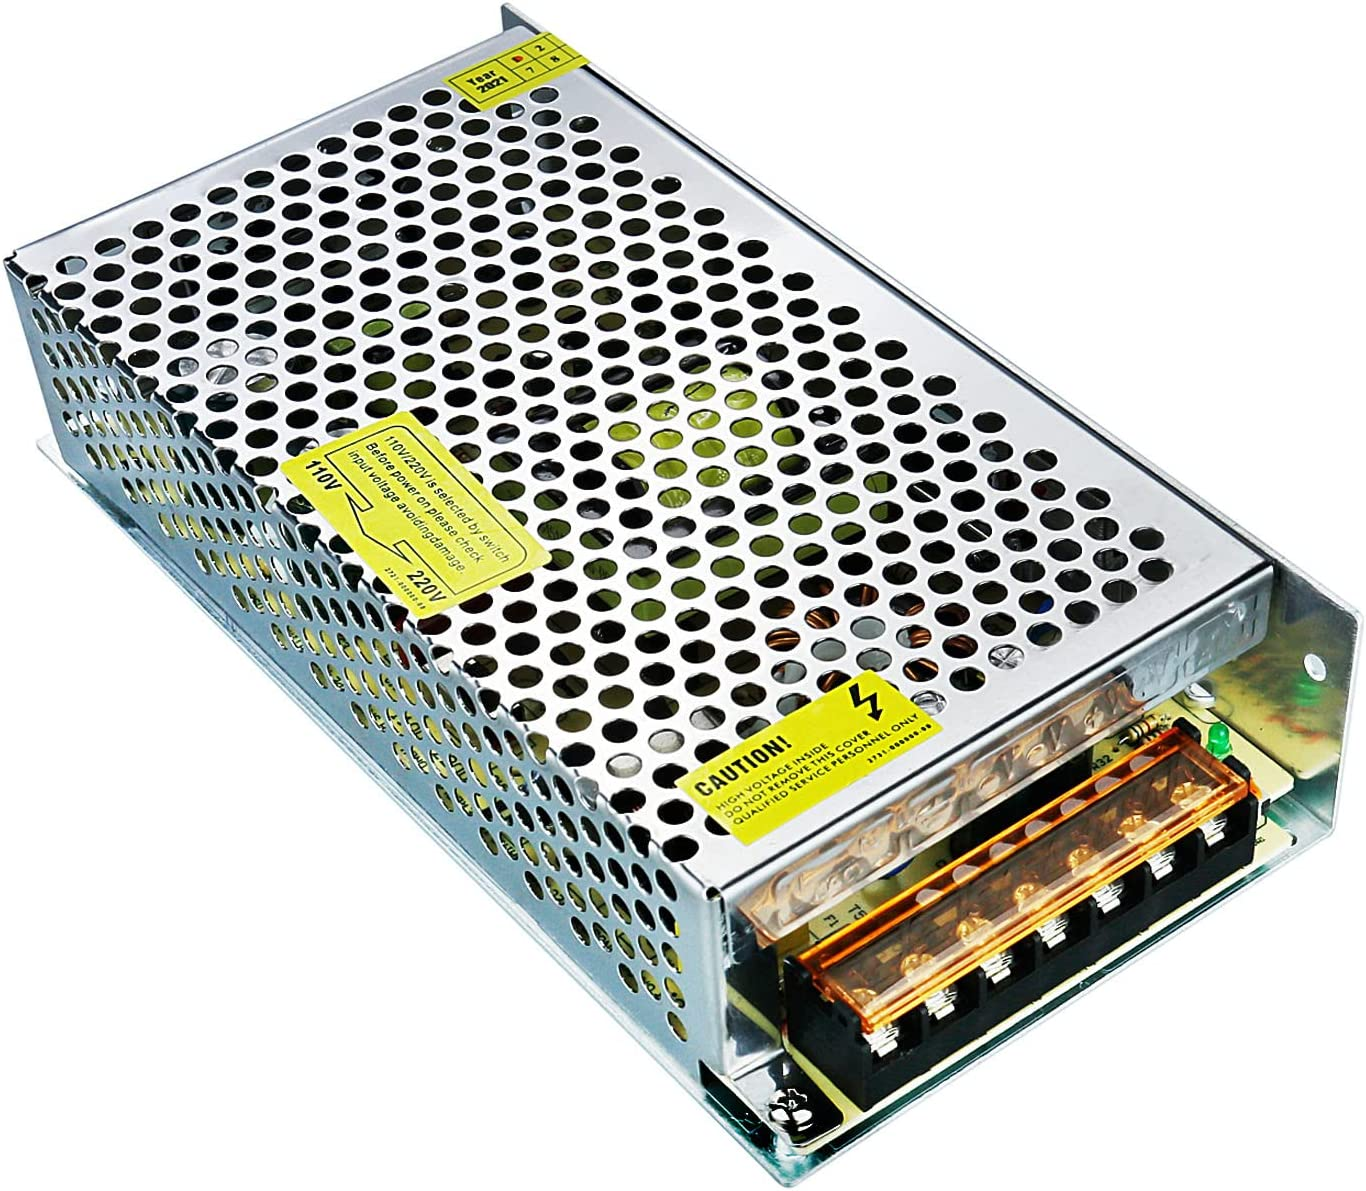
\includegraphics[width=0.45\linewidth ]{figs/pw24v.jpg}}
  \hspace{3cm}
  \subfigure[Cargador de portátil genérico]{\label{fig:pw19}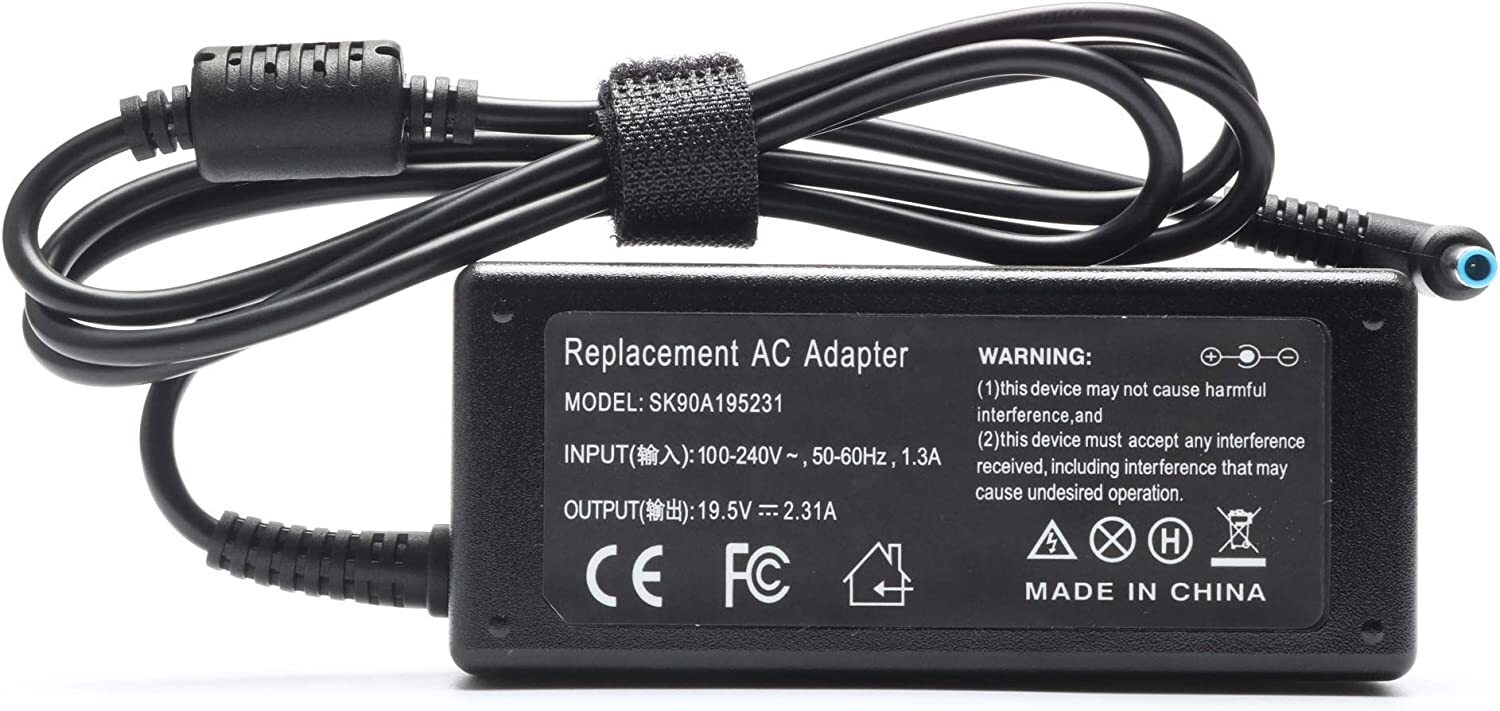
\includegraphics[width=0.55\linewidth]{figs/pw19v.jpg}}
  \caption{Métodos usados para alimentar el robot}
\end{figure}


